\documentclass[11pt]{report}
\usepackage{amsmath}
\usepackage{graphicx}
\usepackage[english]{babel}
\usepackage[labelfont=bf]{caption}
\usepackage{subcaption}
\usepackage{listings}
\usepackage{appendix}

\usepackage{hyperref}
\hypersetup{
    colorlinks,
    citecolor=black,
    filecolor=black,
    linkcolor=black,
    urlcolor=black
}
\usepackage{fancyhdr} % Headers and footers
\pagestyle{fancy} % All pages have headers and footers
\fancyhead{} % Blank out the default header
\fancyfoot{} % Blank out the default footer
\fancyhead[C]{\leftmark} % Custom header text
\fancyfoot[RO,LE]{Page \thepage} % Custom footer text
\fancyfoot[LO,RE]{Shifman \& Cole}

\graphicspath{ {/Users/Chris/repos/modeling_final/TeX/images/} } % hard coded mine, sorry about that
\renewcommand{\headrulewidth}{2pt}
\renewcommand{\footrulewidth}{1pt}


% create a new env for the dedication box - just for you Aaron
\newenvironment{dedication}
  {\clearpage           % we want a new page
   \thispagestyle{empty}% no header and footer
   \vspace*{\stretch{1}}% some space at the top 
   \itshape             % the text is in italics
   \raggedleft          % flush to the right margin
  }
  {\par % end the paragraph
   \vspace{\stretch{3}} % space at bottom is three times that at the top
   \clearpage           % finish off the page
  }



\title{\vspace{-15mm}\fontsize{24pt}{10pt}\selectfont\textbf{Extending the Fitzhugh Nagumo Excitable Tissue Model to Myocardial Necrosis}} % Article title

\author{
\large
\textsc{Aaron R. Shifman, Christopher B. Cole}\thanks{BIO4134 Final Project}\\[2mm] % Your name
\normalsize University of Ottawa \\ % Your institution
\vspace{-5mm}
}
\date{}

%----------------------------------------------------------------------------------------

\begin{document}

\maketitle % Insert title

\thispagestyle{fancy} % All pages have headers and footers

%\tableoffigures

\begin{dedication}
``In general, throughout the work, what is new is not good; and what is good is not new'' - \textbf{Reverend Martin Sherlock}, 1781 
\end{dedication}

\begin{abstract}

Neuroscience frequently relies on robust mathematical models to simulate and investigate trends in neuromechanics and signal propagation. We propose an examination of the Fitzhugh-Nagumo model, and additionally propose a modified extension of this model to account for necrosis of cardiac cells. We use this model to investigate case studies in myocardiac necrosis and examine the effect of necrosis on a one dimensional cardiac model. 
\end{abstract}


\newpage

\tableofcontents

\newpage

\listoffigures

\newpage

\chapter{The Fitzhugh-Nagumo Model}

The modelling of neurons and associated action potentials started in the early 1900s with the ``integrate and fire'' model.$^1$ In 1952, Hodgkin and Huxley created a biologically relevant 4 dimensional system of equations to describe neuron dynamics at a point.$^2$ While very interesting to biologists, mathematicians found the model too difficult to systematically study. In 1961 Richard Fitzhugh created a 2D caricature of the Hodgkin Huxley model (activation and recovery) using a modified Van-der-Pol oscillator.$^3$ This model has been both well studied and well characterized. Additionally, it has found many uses in cardiac models due to its simplicity and similarity in shape to a cardiac action potential. 

The Hodgkin Huxley equations described how neuronal membrane voltage changed over time, given a large number of parameters. 

$$ \begin{aligned} C_m \frac{dV}{dt} &= I_m = I_{Na} + I_{K} + I_l \\ I_x &= \bar{G_x}p_{open}(V_m-E_x); x\in\{Na,K,l\}\\ p_{open_{K}} &= n^4, \, p_{open_{Na}} = m^3h\\ p_{open_{l}} &\equiv 1\\ \frac{dx}{dt} &= \alpha_x(V)(1-x)-\beta_x(V)x; x\in{m,n,h} \end{aligned} $$

This model is impossible to solve analytically, and quite difficult to explore numerically due to both the high dimensionality of the system and the large number of parameters. In studying hyperplanes through the 4D phase space, Nagumo noticed that all planes of activation and recovery variables had a similar shape, so he tried modeling neuronal activity as a modified Van-der-Pol oscillator (Bonheffer-Van-der-Pol oscillator). This model, while not looking like stereotyped action potentials, has several features of the full hodgkin huxley model such as activation hysteresis and spike blocking. Despite not looking like a neuronal action potential, it closely resembles cardiac action potentials and have since been adapted as one of the de-facto models for cardiac simulations. 


\section{Model Rationale and Variables}

The system presents in the following, non-dimensionalized form. This is not the original Bonheffer-Van-der-Pol model, however it is topologically equivalent and much easier to analyse. All models which follow are non-dimensionalized. 

$$ \begin{aligned} \frac{dV}{dt} &= V(\alpha+V)(1-V) -W + z \\
\frac{dW}{dt} &= \beta V-cW \end{aligned} $$

In this model $V$ - in general - represents activation, and in an excitable tissue context represents voltage. and $W$ - in general represents recovery, and has no realistic interpretation in a biological context, it would be the sum of all positive (with regard to the cell) currents. There are four parameters in the model, $\alpha$, $\beta$, $c$, and $z$. Of the four parameters, we have significant interest in $z$, as it will determine the bifurcation of the model. Neurologically, $z$ represents the direct current (DC) offset from experimentally injected current of the neuron under study. In our extension to this model, we will replace $z$ with a gap junctional current from coupled cells (see section \ref{sub:coupled_oscillators}). The additional parameters $\alpha$, $\beta$, and $c$ represent ``rate - like'' constants which determine oscillator traits such as amplitude, frequency, duty cycle, and excitability.


\section{Purpose of Model and Examination}

This model, a simplification of the original Hodgkin Huxley model, intends to model spiking cardiac neurons. Tuning the individual parameters can adapt the model to fit various states and conditions which may be investigated by researchers. Various combinations of parameters can also model neuronal behaviors such as bursting and chattering. These models can be put together to form multi-dimensional models of neuron trends. The state of the neuron relies on the $z$ parameter. 
In this project, we plan to evaluate the stability of system at rest and with regards to the bifurcation parameter $z$. We plan to evaluate how the system responds and bifurcates with regards to this parameter, and interpret these stabilities biologically. 


\begin{figure}[!ht]
  \caption{Time series of $V$ and $W$ following the Fitzhugh Nagumo model. $\alpha = 0.01, \beta = 0.5,c = 0.1,z = 0.5$}
  \centering
    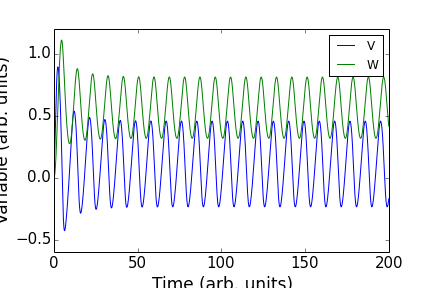
\includegraphics[width=0.75\textwidth]{model}
\end{figure}

Initially, we present a naive time series of the model. We notice that with the set of parameters presented in Eugene Izhikevich 2006, the system oscillates in a stable limit cycle. These parameters, utilized throughout the rest of this report unless otherwise noted, are as follows:

$$ \begin{aligned} \alpha &= 0.01 \\ \beta &= 0.5 \\ c &= 0.1 \\ z &= 0.5 \end{aligned} $$

Using the above parameters, we plot the system on the interval $0 < t \leq 200$ with arbitrary units for time. Note that the system is solved through an adaptive solver \textbf{odeint} in Python 2. 


\section{Model Classification} % (fold)
\label{sub:model_classification}

We classify the system according to the criterion established by Haefner et. al $^{3}$ and find the model is:

\begin{enumerate}
	\item \textbf{Mechanistic} rather than phenomenological. FN models neural dyanmics as a function of individual processes acting on the neuron, including terms analagous to the DC offset, excitation, and relaxation. In this way, the model details the process of neural excitation and is process oriented.
	\item \textbf{Dynamic} rather than static. The system models excitation and relaxation as a function of time, and is thus a dynamic model.
	\item \textbf{Continuous} rather than discrete. The model uses time on an arbitrary scale as a continuous variable, instead of taking predefined ``steps''. In this way, the system uses time continuously. 
	\item \textbf{Spatially homogenous} rather than spatially heterogeneous. The model contains no explicit description of space, and is thus homogeneous. 
	\item \textbf{Deterministic} rather than stochastic. All terms in the model are entirely predictable given initial conditions and no events based on chance occur. Thus the model is deterministic. 
\end{enumerate}

% subsection dimensionalization (end)
\section{Stability Analysis} % (fold)
\label{sub:stability_analysis}

Taking our model such that:

$$\begin{aligned}
f(x) &= \dot{V} = V(\alpha + V)(1-V) -W +z \\
g(x) &= \dot{W} = \beta V -cW
\end{aligned}
$$

We compute the Jacobian Matrix $\vec{J}$:


$$
\vec{J} = \begin{bmatrix}
    \frac{\partial f}{\partial{V}} & \frac{\partial f}{\partial{W}} \\
    \frac{\partial g}{\partial{V}} & \frac{\partial g}{\partial{W}} \\
\end{bmatrix} = 
\begin{bmatrix}
    −2\alpha V+\alpha+(2 - 3V)V & -1 \\
    \beta & -c \\
\end{bmatrix}
$$


Taking $\alpha,\beta,c$ equal to 0.01,0.5,0.1 respectively,
$$
\begin{bmatrix}
    −0.02V+(2−3V)V+0.01 & -1 \\
    0.5 & -0.1 \\    
\end{bmatrix}
$$

This implies that eigenvalues $\lambda_{1,2}$ may be complex or not. 

Eigenvalues 1 and 2 as follows

$$ \lambda_{1,2} \approx \begin{bmatrix} 0.5(-3V^2 - 1.98V + \sqrt{ 9V^4 + 11.88 V^3 + 3.2604 V^2 - 0.4356 V - 1.9879 } - 0.09) \\ 0.5(-3V^2 - 1.98V - \sqrt{ 9V^4 + 11.88 V^3 + 3.2604 V^2 - 0.4356 V - 1.9879 } - 0.09) \end{bmatrix} $$

with corresponding eigenvectors

$$ v_{1,2} \approx \begin{bmatrix} 0.11 + 1.98V - 3V^2 + \sqrt{ 9V^4 + 11.88 V^3 + 3.2604 V^2 - 0.4356 V - 1.9879} & 1 \\ 0.11 + 1.98V - 3V^2 - \sqrt{ 9V^4 + 11.88 V^3 + 3.2604 V^2 - 0.4356 V - 1.9879} & 1 \end{bmatrix} $$

We plot the eigevalues to describe their dynamics. 

\begin{figure}[!ht]
  \caption{Eigenvalues as a function of the steady state $V^*$ for $z$.  $\alpha = 0.01, \beta = 0.5,c = 0.1,z \in [0,5]$ }
  \centering
    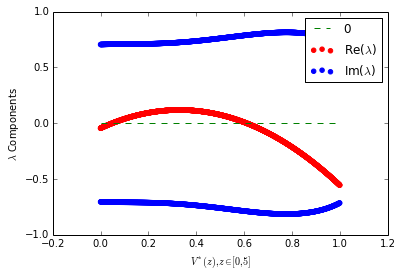
\includegraphics[width=0.75\textwidth]{eig}
\end{figure}

Note that the vertical axis of the above plot corresponds to the value of the eigenvalue, while the lower horizontal axis denotes the value of the steady state $V^*$ for $z \in [0,5]$ while the upper horizontal axis corresponds to the $z$ value itself.

There is an observable bifurcation when the real component of the eigenvalue passes from negative to positive just above $V^*(z) = 0$, and when the real component of $\lambda$ passes from positive to negative, at just below $V^*(z) = 0.6$. To confirm these values we plot a low resolution bifurcation:


\begin{figure}[!ht]
  \caption{Low resolution bifurcation diagram of the system. Stable limit of $V$ plotted on the vertical axis while $z$ is depicted on the horizontal. $\alpha = 0.01, \beta = 0.5,c = 0.1,z \in [0,5]$ }
  \centering
    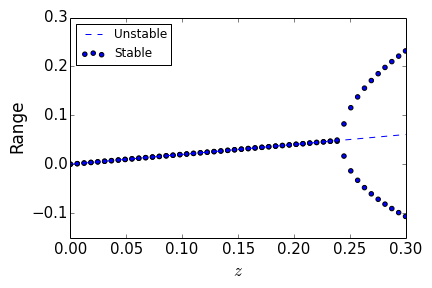
\includegraphics[width=0.75\textwidth]{lbifur}
\end{figure}


and subsequently confirm this with a tigher view of the left bifurcation point.

\begin{figure}[!ht]
  \caption{High resolution bifurcation diagram of the system. Stable limit of $V$ plotted on the vertical axis while $z$ is depicted on the horizontal. $\alpha = 0.01, \beta = 0.5,c = 0.1,z \in [0,5]$ }
  \centering
    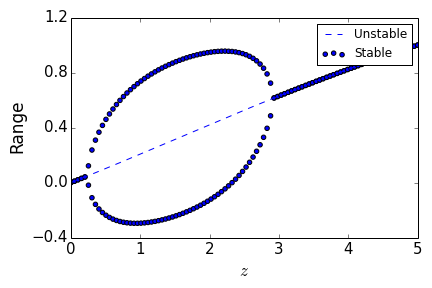
\includegraphics[width=0.75\textwidth]{hbifur}
\end{figure}


This appears to be an example of a Hopf bifurcation point at both of these instances. There is initially a fixed point which is stable, corresponding to no oscillation as well as a pair of complex conjugate eigenvalues. As $z$ increases and reaches the first bifurcation, the fixed point loses stability and the stable limit cycle forms. That is, until $z$ reaches the seconf bifurcation point and the limit cycle collapses back to the single stable fixed point as the real component of the eigenvalue once again becomes negative. We can visualize this stable limit cycle by plotting the phase plane of the system with a stable value of $z = 0.5$.

\begin{figure}[!ht]
  \caption{Phase plane of the FN system. $\alpha = 0.01, \beta = 0.5,c = 0.1,z \in [0,5]$ }
  \centering
    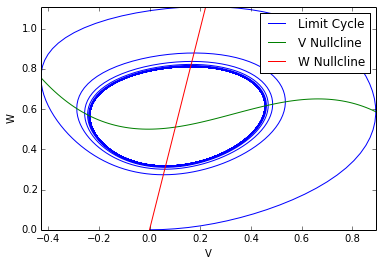
\includegraphics[width=0.75\textwidth]{phase-plane}
\end{figure}

This clearly displays the system oscilating for the appropriate value of $z$. In the following section, we take advantage of this property and modify the $z$ term to incorporate both coupled oscilators and the disease etiology of myocardial necrosis. 




\section{Coupled Oscillators} % (fold)
\label{sub:coupled_oscillators}

The previously described model is useful for observing the dynamics of a single cardiac neuron, however occasionally researchers wish to incorporate several connected neuros in the same system. 

Here we couple neurons, first two, then $n$, in a modified \textbf{synfire} chain. In this network, current is expressed through gap junctions and can only travel in one direction. Current flows from the first neuron ($N_1$) to the second neuron $N_2$ and sequentially through neurons $N_i$ to $N_n$. When the current reaches the final neuron $N_n$, it is returned to the original neuron $N_1$. Conceptually, the model can be thought of as a circular path, though in reality this is a specific kind of boundary condition and has no implications for the true geography of the system. 

From here on, we present only $V$ and omit $W$ from our analysis, as it is not advantageous to track both quantities. In order to couple neurons, we propose the following model to couple neurons $N_A$ and $N_B$:


We connect oscillators with a gap junctional current ($I_g = G_g(\Delta V)$). For a population of $n$ oscillators $\Omega$, with members $\omega_i; i\in \textbf{N}; 1\leq i\leq n$. If $\omega_i$ is connected to $x; x\subset\Omega$, then the gap junctional current to $\omega_i$ is $\sum_{x} G_{x,i}(V_i-V_x)$

In the case of 2 oscillators ($A$ and $B$)

$$ \begin{aligned} \frac{dV_A}{dt} &= V(\alpha +V_A)(1-V_A) -W_A + G_g(V_A-V_B) + z_A\\ \frac{dV_B}{dt} &= V(\alpha +V_B)(1-V_B) -W_B + G_g(V_B-V_A) +z_B\\ \frac{dW_A}{dt} &= \beta V_A - cW_A\\ \frac{dW_B}{dt} &= \beta V_B - cW_B
\end{aligned} $$

Using the above model, we construct a system with two coupled neurons and graph their time series on the interval $t \in [0,200]$. Observe that both neurons are out of phase by a constant amount.


\begin{figure}[!ht]
  \caption{Two coupled neurons. $\alpha = 0.01, \beta = 0.5,c = 0.1,z \in [0,5]$ }
  \centering
    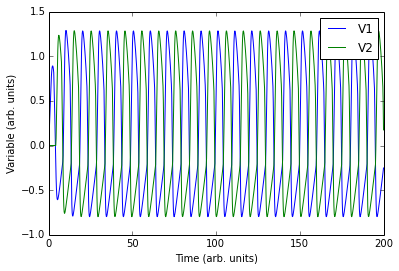
\includegraphics[width=0.75\textwidth]{2couple}
\end{figure}

We further extend the model to couple $n$ neurons. 

\begin{figure}[!ht]
  \caption{$n=5$ coupled neurons. $\alpha = 0.01, \beta = 0.5,c = 0.1,z \in [0,5]$ }
  \centering
    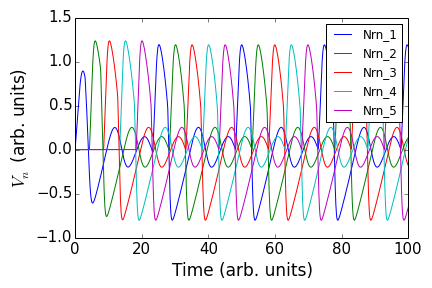
\includegraphics[width=0.75\textwidth]{ncouple}
\end{figure}

Note that the above has used paramters such that the stable limit cycle is sustained. We can use this extension to the FN model in order to answer biologically relevant questions about myocardial necrosis in the following section. 
% subsection coupled_oscillators (end)


Additionally, we describe the frequency change as a function of the number of neurons in the system. As frequency is defined by $\frac{1}{period}$, with increasing number of neurons, frequency decreases. At the extreme, as $n \rightarrow \infty, f \overset{a.s.}{\rightarrow} 0$.



\begin{figure}[!ht]
  \caption{System frequency as a function of neuron count. $\alpha = 0.01, \beta = 0.5,c = 0.1,z=0.5$ }
  \centering
    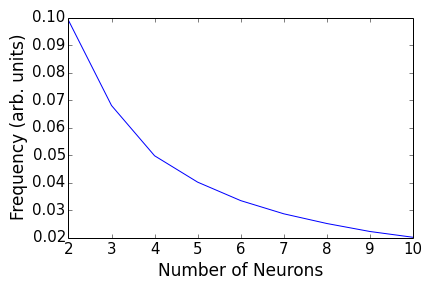
\includegraphics[width=0.75\textwidth]{freq_static}
\end{figure}

Note that the coupled system behaves as expected. 



%end original model, begin extension

\chapter{Modelling Myocardial Necrosis} 


\section{Translational Perspective} %how the model relates to disease

The heart serves a vital role in many organisms. The timely and regular delivery of oxygenated blood is essential to survival, and thus any decrease from optimum efficiency is of consequence. Investigations into potential mechanistic explainations and modeling of this degradation are highly interesting in the context of both accute and chronic cardiac disease.

In particular, myocardial necrosis can be caused by accute oxygen deprivation of myocardial tissues, commonly experienced during a heart attack. Other potential etiologies stem from depriving this tissue of the blood it requires; dangerous increase in physical stresses, coronary artery disease, and accute hemerage all have the potential to play into cardiac necrosis, perhaps in tandem. 

In our investigation into the decreasing efficiency of a heart-like system, we will model several scenarios that may be of consequence to sufferers of cardiac necrosis. In particular, we study two cases. The first, static necrosis, closely resembles a short term or acute stress on myocardial tissue, be it a myocardial infarction or trauma. We will investigate how the distribution of necrosis affects the system as a whole through the FN model. Through a translation lens, this equates to the decrease in efficiency as a consequence of various kinds of trauma. The second case will be a slowly increasing level of necrosis. This more closely resembles coronary artery disease, which has the potential to starve the tissues of oxygen for many years, slowly leading to health deficits in older age. We study the approximate timeframe for simulated tachycardia, or dangerously low heart beat. 

Throughout the investigation, we refer to a cell's necrosis burden as analagous to a protein build up, though this simply refers to the degree of degredation for that specific cell.

Our proposed extension to the FN model plans to shed light on the geneisis, progression, and finally the consequences of myocardial necrosis. 

\section{Necrosis Propagation}

As part of the normal cell cycle, programmed cell death (apoptosis) exists and it serves several purposes. In most cases, it is both irreversible and adaptive (beneficial) for the organism. However in some cases, apoptosis can occur accidentally in which case an irreversible destruction of the cell will occur. In our model, we assume that necrosis is a function of an underlying accumulation of pro-apoptotic proteins, potentially introduced as a byproduct of disease. As such, necrosis is a continuous state of each cell. For cell $i$ of $n$, define pro-necrotic burden as $\nu_i$, with total burden of the system equal to $\frac{\sum^n_{i=1} \nu_i}{n}=\frac{1}{n} \sum^n_{i=1} \nu_i$. Note that $\nu_{1}, ..., \nu_{n} \in [0,1]$ and is a monotonically increasing function with respect to time. 

Starting with the Fitzhugh Nagumo model equivalent
\begin{align}
\frac{dV}{dt} &= V(\alpha +V)(1-V) -W +z\\
\frac{dW}{dt} &= \beta V - cW
\end{align}



\section{Static Disease Burden} % (fold)
\label{sub:static_disease_burden}

Recall that $\nu_i$ is defined as the proportion of channels damaged or lost in neuron $N_i$. We define this as the necrotic burden of neuron $N_i$. In this section we study the effects of an acute injury which leaves the patient with a sudden decrease in neuronal efficiency analogous to a sudden addition of the $\nu_i$ term. We first develop a model for this situation, then use this model to investigate how the distribution of necrotic burden affects the system.

\subsection{Disease Model} % (fold)
\label{sub:disease_model}

% subsection disease_model (end)

For the coupled oscillators representing cardiac myocytes, as the cells die through an apoptotic pathway, a fraction of their gap junctions $\nu \in [0,1]$ will be destroyed, through cell decay.

In order to model disease, each myocyte will have a corresponding $\nu$ term, such that

\begin{align}
\frac{dV_A}{dt} &= V(\alpha +V_A)(1-V_A) -W_A + (1-\nu_A) G_g(V_A-V_B) + z_A\\
\frac{dV_B}{dt} &= V(\alpha +V_B)(1-V_B) -W_B + (1-\nu_B) G_g(V_B-V_A) +z_B
\end{align}
With increasing $\nu$, the cell becomes less responsive to its coupled partners.

We present the above model for both 2 (as a test case) and $n$ coupled neurons with static necrosis term $\nu_i$.

\begin{figure}[!ht]
  \caption{Static disease model in two neurons. $\alpha = 0.01, \beta = 0.5,c = 0.1,z = 0.5, \nu_1 = 0.5, \nu_2 = 0$ }
  \centering
    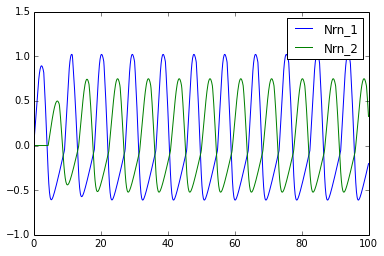
\includegraphics[width=0.75\textwidth]{2stat}
\end{figure}


\begin{figure}[!ht]
  \caption{Static disease model in $n=5$ neurons. $\alpha = 0.01, \beta = 0.5,c = 0.1,z = 0.5, \nu_1 = 0.1, \nu_2 = 0.1, \nu_3 = 0.1, \nu_4 = 0.1, \nu_5 = 0.1$ }
  \centering
    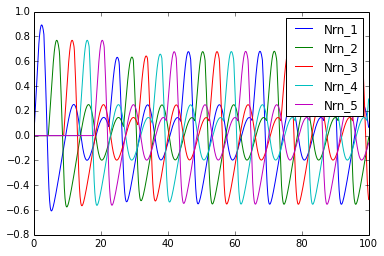
\includegraphics[width=0.75\textwidth]{nstat}
\end{figure}


We use this model to answer biologically relevant questions. 

% subsection development_of_model (end)

\subsection{Dispersion of Necrosis} % (fold)
\label{sub:dispersion_of_necrosis}

% subsection distribution_of_necrosis (end)

We initially investigate how the distance between disease burdens may affect the cellular system.

\textbf{Lemma:} $\nu_i=1$ is a trivial solution which will destroy the system every time, so from this point onwards it is excluded from all analyses.

\textbf{Proof:} Let $\Omega$ be a population of $n$ neurons called $N_1, N_2, ..., N_{n-1}, N_n$. For any $1 \leq i \leq n$, if $\nu_i=1$, $1-\nu_i=0$, and accordingly $(1-\nu_i) G_g(V_i-V_{i+1)}) + z_i=0$ because $z_i=0$ for any time above the initial impulse. Thus, $z_{eff} = (1-\nu_i) G_g(V_i-V_{i+1}) + z_i = 0$ or the effective $z$ which is acting on the system is $0$ for any $\nu_i=1$. Following this logic, if $z_{eff}=0$ for any neuron $i$, $N_i$ will have a negative real component to its eigenvalue $\lambda$, and thus will have only one steady fixed point solution and not enter a stable limit cycle. Because $N_i$ will be fixed, $N_{i+1}$ will become fixed, and the effect will propegate throughout the system $\Omega$. In this way, $\nu_i=1$ for any $1 \leq i \leq n$ will be a trivial solution to the system.

We hypothesize that the distance between disease burdens should not play a role in how effective they are in diminishing the system's efficacy. 

To lend evidence to our hypothesis, we construct two systems $A$ and $B$, labelled accordingly. In system $A$, we impose a disease burden on dispersed cells. We damage $N_1$ and $N_3$, leaving all others unaffected ($\nu_i = 0$ for all others). We define $\nu_1 = 0.5$ and $\nu_3 = 0.5$. We plot the solution to the system and observe that, though there are ramifications and the system appears more spastic, it is systained. In system $B$, we impose sequential burdens such that $\nu_1 = 0.5$ and $\nu_2 = 0.5$, leaving all others unburdened ($\nu_i = 0$). In this case, we observe a rapid collapse of the system. 


\begin{figure}
    \centering
    \begin{subfigure}[b]{0.48\textwidth}
        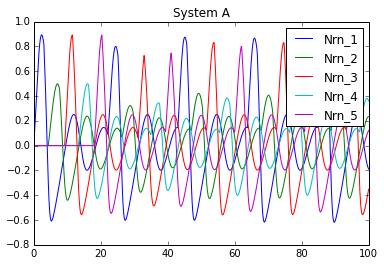
\includegraphics[width=\textwidth]{statA}
        \caption{Dispersed necrotic burden in a static disease model. $\nu_{1,3} = 0.5, \nu_{2,4,5} = 0, \alpha = 0.01, \beta = 0.5,c = 0.1$}
        \label{fig:statA}
    \end{subfigure}
    \hfill %add desired spacing between images, e. g. ~, \quad, \qquad, \hfill etc. 
      %(or a blank line to force the subfigure onto a new line)
    \begin{subfigure}[b]{0.48\textwidth}
        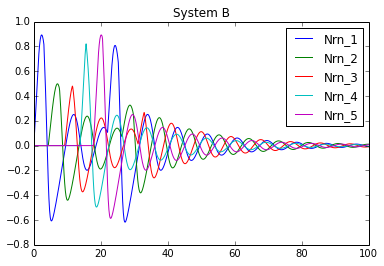
\includegraphics[width=\textwidth]{statB}
        \caption{Sequential necrotic burden in a static disease model. $\nu_{1,2} = 0.5, \nu_{3,4,5} = 0, \alpha = 0.01, \beta = 0.5,c = 0.1$}
        \label{fig:statB}
    \end{subfigure}
    \caption{Examining the effects of dispersion on system performance in a static model. }\label{fig:dispersion}
\end{figure}


We interpret these results at the end of this section. 

\subsection{Density of Necrosis} % (fold)
\label{sub:density_of_necrosis}

% subsection density_of_necrosis (end)


We proceed to investigate whether few large burdens or multiple smaller burdens may affect the system more. We construct two systems $A$ and $B$ such that $\sum^n_{i=1} \nu_{Ai} = \sum^n_{i=1} \nu_{Bi}$ but choose to minimize the burden in each cell for system $A$, while we concentrate it in a single neuron for system $B$. We chose to assign $\nu_{1,2,3,4,5}= 0.15$ for system $A$ and $\nu_3 = 0.75$ for system $B$. System $A$ appears to sustain itself while system $B$ rapidly collapses. We interpret these results in the following section.

\begin{figure}
    \centering
    \begin{subfigure}[b]{0.48\textwidth}
        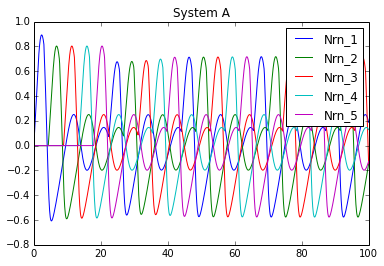
\includegraphics[width=\textwidth]{statA2}
        \caption{Minimal necrotic burden per neuron in a static disease model. $\nu_{1,2,3,4,5} = 0.15, \alpha = 0.01, \beta = 0.5,c = 0.1$}
        \label{fig:statA2}
    \end{subfigure}
    \hfill %add desired spacing between images, e. g. ~, \quad, \qquad, \hfill etc. 
      %(or a blank line to force the subfigure onto a new line)
    \begin{subfigure}[b]{0.48\textwidth}
        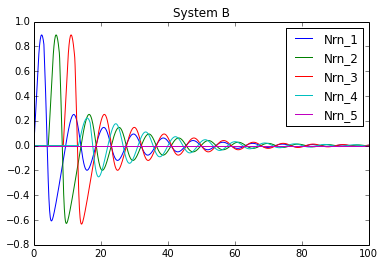
\includegraphics[width=\textwidth]{statB2}
        \caption{Maximal necrotic burden in a single neuron for a static disease model. $\nu_{3} = 0.75, \nu_{1,2,4,5} = 0, \alpha = 0.01, \beta = 0.5,c = 0.1$}
        \label{fig:statB2}
    \end{subfigure}
    \caption{Examining the effects of density on system performance in a static model.}\label{fig:density}
\end{figure}


\subsection{Discussion} % (fold)
\label{sub:discussion}

From the analsysis above, we lend support to the ideas that the worst (most destructive) necrosis in a system would be a clustered, concentrated increase in necrosis. In practice, this means that a sudden traumatic incident such as an acute occlusion of a cardiac blood vessel would have a must more direct impact than a chronic condition slowly necrotizing tissue.

More sophisticated mehthods would be required to ascertain the bounds on these conditions due to the high dimensionality of the system. At this point of the analysis we can only lend evidence to the above ascertation. We continue this analysis with the development of a dynamic evolution of the $\nu$ necrosis burden. 

% subsection discussion (end)


\section{Dynamic Disease Burden} % (fold)
\label{sub:dynamic_disease_burden}

In order to extend this model to model cardiac necrosis, we use the previously described coupling and staic model, adding $\nu_i$ as an ordinary differential equation describing the dampening on neuron $i$ ($N_i$). In the present simplication, $\nu_i$ will depend only on time. Define $\nu_{0i}$ as the \textit{a priori} necrotic burden of $N_i$. 

\subsection{Disease Model} % (fold)
\label{sub:disease_model}

% subsection disease_model (end)

We wish to construct a model of $\nu_{i}$ evolution where, eventually, the disease will destroy the cell. Thus, we wish to have 1 (complete dampening) as a stable steady state. Additionally, we require that any concentration of $\nu_{0i}$ will eventually lead to cell death. We chose the model

$$ \frac{d \nu_i}{dt} = \dot{\nu} = \nu_i (1 - \nu_i) $$

Giving a distribution of the rate of change corresponding to the following:

\begin{figure}[!ht]
  \caption{Differential Equation describing the evolution of $\nu_i$ with respect to time. }
  \centering
    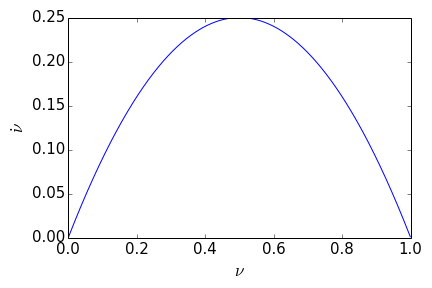
\includegraphics[width=0.75\textwidth]{dynamic}
\end{figure}


Note that in this model, $\nu_i=0$ is an unstable steady state while $\nu=1$ is a stable steady state. This is desirable for the model, and intuitivly means that any amount of $\nu_i$ will eventually go to 1 and stop the system. 

We demonstrate the above model in a two neuron system.

\begin{figure}[!ht]
  \caption{Dynamic disease model in two neurons. $\alpha = 0.01, \beta = 0.5,c = 0.1,z = 0.5, \nu_1 = 0.01, \nu_2 = 0$ }
  \centering
    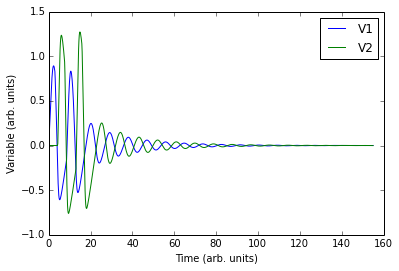
\includegraphics[width=0.75\textwidth]{2dyn}
\end{figure}


And also in a system with $n=5$ neurons.

\begin{figure}[!ht]
  \caption{Dynamic disease model in five neurons. $\alpha = 0.01, \beta = 0.5,c = 0.1,z = 0.5, \nu_1 = 0.01, \nu_2 = 0, \nu_3 = 0, \nu_4 = 0, \nu_5 = 0$ }
  \centering
    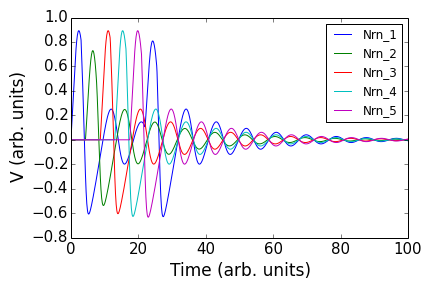
\includegraphics[width=0.75\textwidth]{ndyn}
\end{figure}

\subsection{Dispersion of Necrosis} % (fold)
\label{sub:dispersion_of_necrosis}

We repeat the above analysis for the dynamic system. First we create a system $A$ with initial dispursed necrosis such that $\nu_{1,3} = 0.1$ and $\nu_{2,4,5} = 0$. We additionally construct a second system $B$ such that the initial necrosis is clustered, $\nu_{1,2} = 0.1$ and $\nu_{3,4,5} = 0$. We plot the solution to the system and observe no radical difference between the two systems.

\begin{figure}
    \centering
    \begin{subfigure}[b]{0.48\textwidth}
        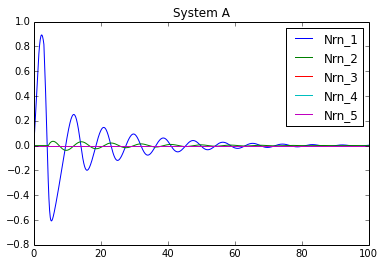
\includegraphics[width=\textwidth]{dynA}
        \caption{Dispersed necrotic burden in a dynamic disease model. $\nu_{1,3} = 0.1, \nu_{2,4,5} = 0, \alpha = 0.01, \beta = 0.5,c = 0.1$}
        \label{fig:statA}
    \end{subfigure}
    \hfill %add desired spacing between images, e. g. ~, \quad, \qquad, \hfill etc. 
      %(or a blank line to force the subfigure onto a new line)
    \begin{subfigure}[b]{0.48\textwidth}
        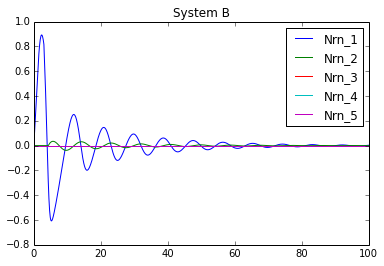
\includegraphics[width=\textwidth]{dynB}
        \caption{Sequential necrotic burden in a dynamic disease model. $\nu_{1,2} = 0.1, \nu_{3,4,5} = 0, \alpha = 0.01, \beta = 0.5,c = 0.1$}
        \label{fig:statB}
    \end{subfigure}
    \caption{Examining the effects of dispersion on system performance in a dynamic model. }\label{fig:dispersion}
\end{figure}

We discuss implications of the above in the next section. 


\subsection{Density of Necrosis} % (fold)
\label{sub:density_of_necrosis}


Additionally, we examine the effect of necrosis density on system performance. We create a system $A$ where all of the initial necrosis is concentrated in a single neuron such that $\nu_3 = 0.5$ and $\nu_{1,2,4,5} - 0$. We compare this to system $B$ where we give each neuron a smaller level of disease burden such that $\sum^n_{i=1} \nu_{Ai} = \sum^n_{i=1} \nu_{Bi}$. In system $B$ we define $\nu_{1,2,3,4,5} = 0.1$.


\begin{figure}
    \centering
    \begin{subfigure}[b]{0.48\textwidth}
        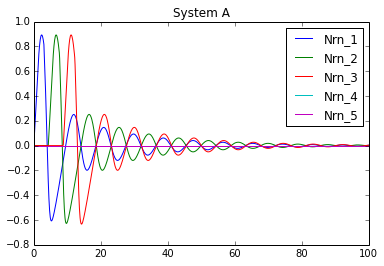
\includegraphics[width=\textwidth]{dynA2}
        \caption{Minimal necrotic burden per neuron in a dynamic disease model. $\nu_{1,2,3,4,5} = 0.1, \alpha = 0.01, \beta = 0.5,c = 0.1$}
        \label{fig:dynA2}
    \end{subfigure}
    \hfill %add desired spacing between images, e. g. ~, \quad, \qquad, \hfill etc. 
      %(or a blank line to force the subfigure onto a new line)
    \begin{subfigure}[b]{0.48\textwidth}
        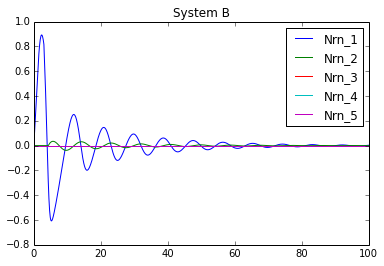
\includegraphics[width=\textwidth]{dynB2}
        \caption{Sequential necrotic burden in a dynamic disease model. $\nu_{3} = 0.5, \nu_{1,2,4,5} = 0, \alpha = 0.01, \beta = 0.5,c = 0.1$}
        \label{fig:dynB2}
    \end{subfigure}
    \caption{Examining the effects of density on system performance in a dynamic model. }\label{fig:dispersion}
\end{figure}


We interpret the above in the following section.


\subsection{Discussion} % (fold)
\label{sub:discussion}

% subsection discussion (end)

By using our model, we demonstrate that the distribution of initial necrosis does not affect, or at least does not meaningfully effect, the degredation of the system. Additionally we found that a system with lower initial concentrations in many neurons more rapidly destroys the system than a higher initial concentration in a single neuron. 

Intuitively this tells us that a more dispersed illness which is evolving will have a more devastating effect than a locally contained one. 

\section{Conclusion} % (fold)
\label{sec:conclusion}


In summary, we present an examination of the Fitzhugh Nagumo model for relaxation oscillators, a simplication of the original Hodgkin-Huxley. We analyze the stability of this model and provide insight into its dynamics. In addition to the base model, we develop three extensions. Firstly, we develop a method for the coupling of multiple  neurons, allowing us to simulate a modified synfire chain. Using this coupling method, we introduce a new term $\nu$ to represent the proportion of destroyed ion channels as a result of myocardial necrosis. We introduce this term into our coupling extension first as a parameter, and second as differential equation tracking disease progression. We use these extensions to make statements related to disease prognoses and the differences amung various situations. 

The modelling of biological systems represents a crucial cog in the machine developing solutions to medicinal problems. With our extension, we take a further step towards undstanding the etiology of various diseases sharing a genesis involving cardio-hypoxic events such as strokes and acute trauma. Our model has wide implications from myocardial infarction to drug delivery to carcinogenic pathways. More work must be done in this area to correctly model these disease \textit{in silico}. Only by understanding the pathways and processes involved in disease can we hope to combat it, and eventually, to beat it.  

% section conclusion (end)


% subsection static_disease_burden (end)
\chapter{Additional Material} % (fold)
\label{sub:web_app}


\section{Web App} % (fold)
\label{sec:web_app}

% section web_app (end)


\subsection{Description of Model} % (fold)
\label{sub:description_of_model}

In addition to the previous analysis, we present an interactive model to observe the effects of various combinations of parameters. The application, at present, only performs analysis for the static case of the model.

The application is written in the programming language R 3.2.2 and hosted on shinyapps. The app can also be built locally. 

The application uses the forward Euler method for solving differential equations, and the user is invited to see the effects of changing any parameter on the system's behavior. 

% section description_of_model (end)}

\begin{figure}[!ht]
  \caption{Interactive visualization of two coupled neurons following the FN model with extension. }
  \centering
    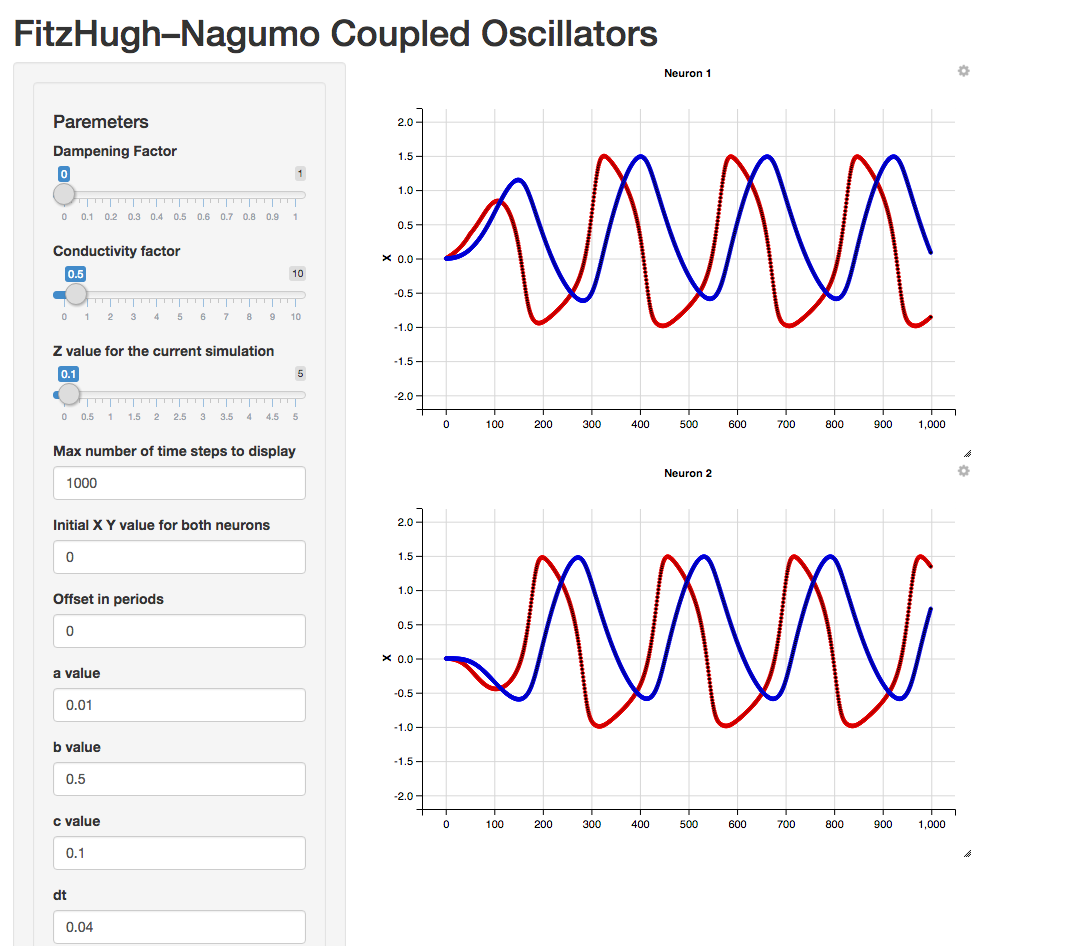
\includegraphics[width=0.75\textwidth]{R}
\end{figure}

% subsection web_app (end)
\newpage

\subsection{Building locally} % (fold)
\label{sub:building_locally}

To build the application locally, clone the git repo to your system and change your directory to the shiny repository. Start R. 

\begin{lstlisting}[language = sh]

$ git clone https://github.com/aaronshifman/modeling_final.git
$ cd modeling_final/shiny 
$ R

\end{lstlisting}

The web app has several dependencies. The following packages must be installed:


\begin{enumerate}
  \item ggvis
  \item shiny
  \item deSolve
\end{enumerate}

Once installed, type RunApp() into the R console. The application will display in a viewer.


\section{Additional Visualizations \& Supporting Information} % (fold)
\label{sec:web_app}


\subsubsection{Dynamic Visualizations} % (fold)
\label{ssub:dynamic_visualizations}

% subsubsection dynamic_visualizations (end)
All of the following visualizations are contained within the following iPython notebook: 

\begin{lstlisting}
  
http://nbviewer.ipython.org/github/aaronshifman/modeling_final/blob/master/ipynb/python%20model%20-%20isolated.ipynb

\end{lstlisting}


\textbf{Figure S1}: Sweep of phase plane for $z \in [0,1]$

\textbf{Figure S2:} Coupling animation

% section \dynamic_visualizations_and_additional_software (end)


\chapter{References} % (fold)
\label{sec:references}

\begin{enumerate}
  \item Abbott, L. . Lapicque’s introduction of the integrate-and-fire model neuron \(1907\). Brain Res. Bull. 50, 303–304 \(1999\).
  \item Hodgkin, A. L., Huxley, A. F. A quantitative description of membrane current and its application to conduction and excitation in nerve. J. Physiol. 117, 500–44 \(1952\).
  \item Haefner, J. W. Models of Systems. Modeling Biological Systems: Principles and Applications \(Springer, 2005\). doi:10.1007/0-387-25012-3\_1
\end{enumerate}


% section references (end)

\end{document}





